
\begin{frame}
\frametitle{Axis encoding: motivación}

\begin{figure}[h]
\centering
\subfloat[\centering $\white$ White]{{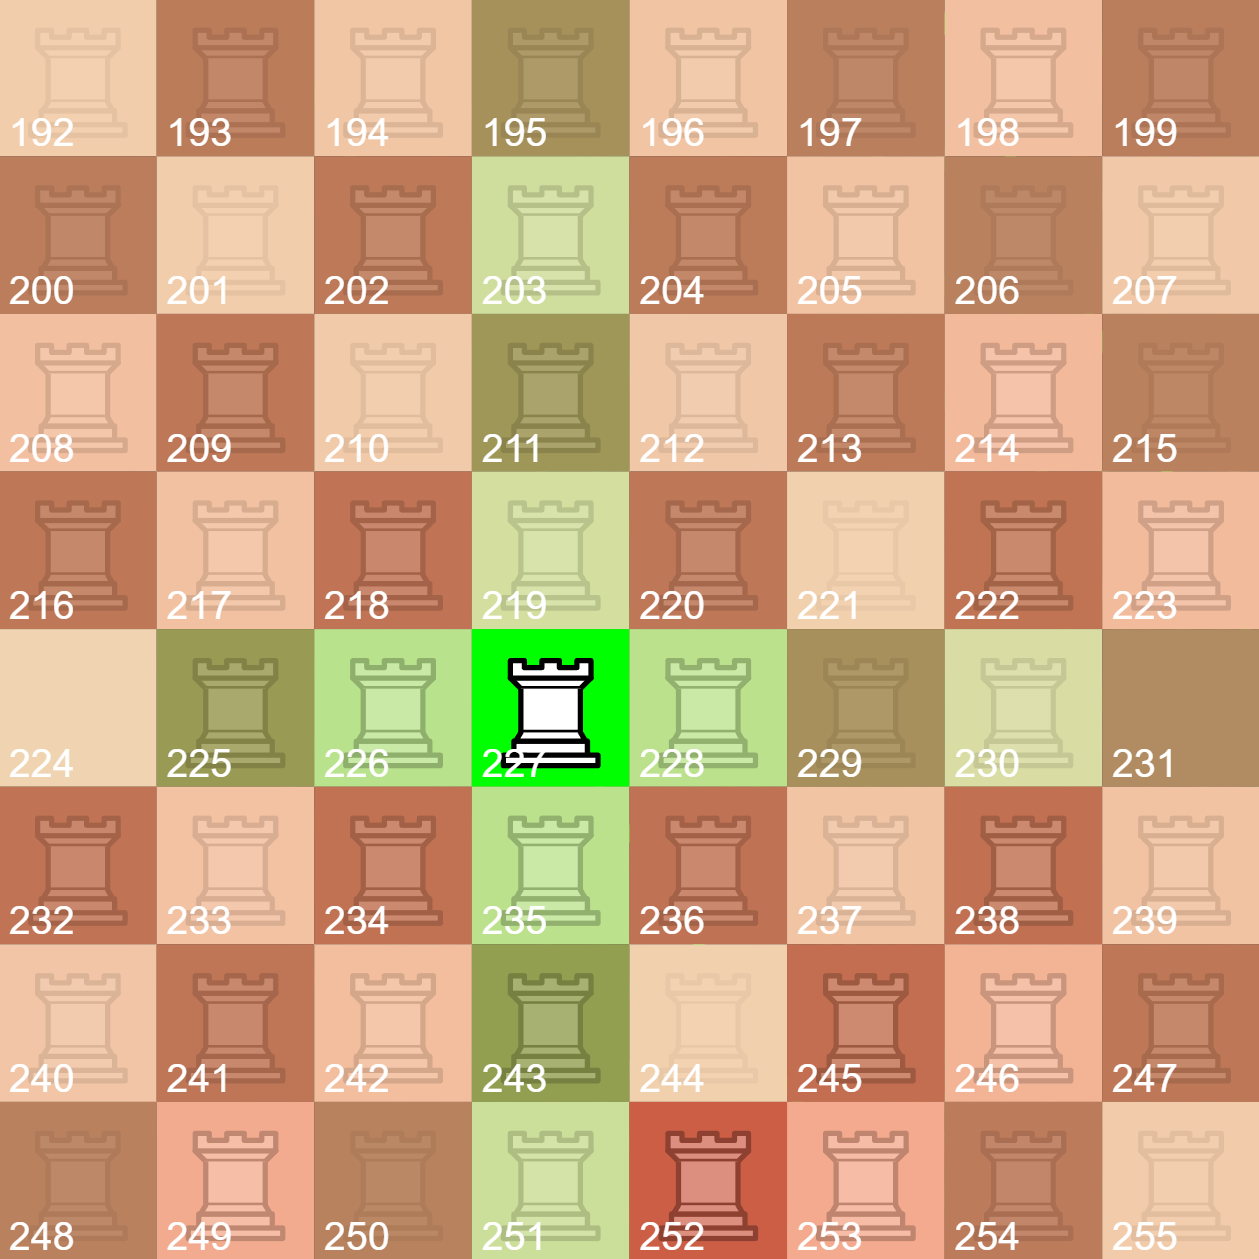
\includegraphics[width=4.4cm]{../assets/results/piece_weights/white_rook_weights.png} }}%
\qquad
\subfloat[\centering $\black$ Black]{{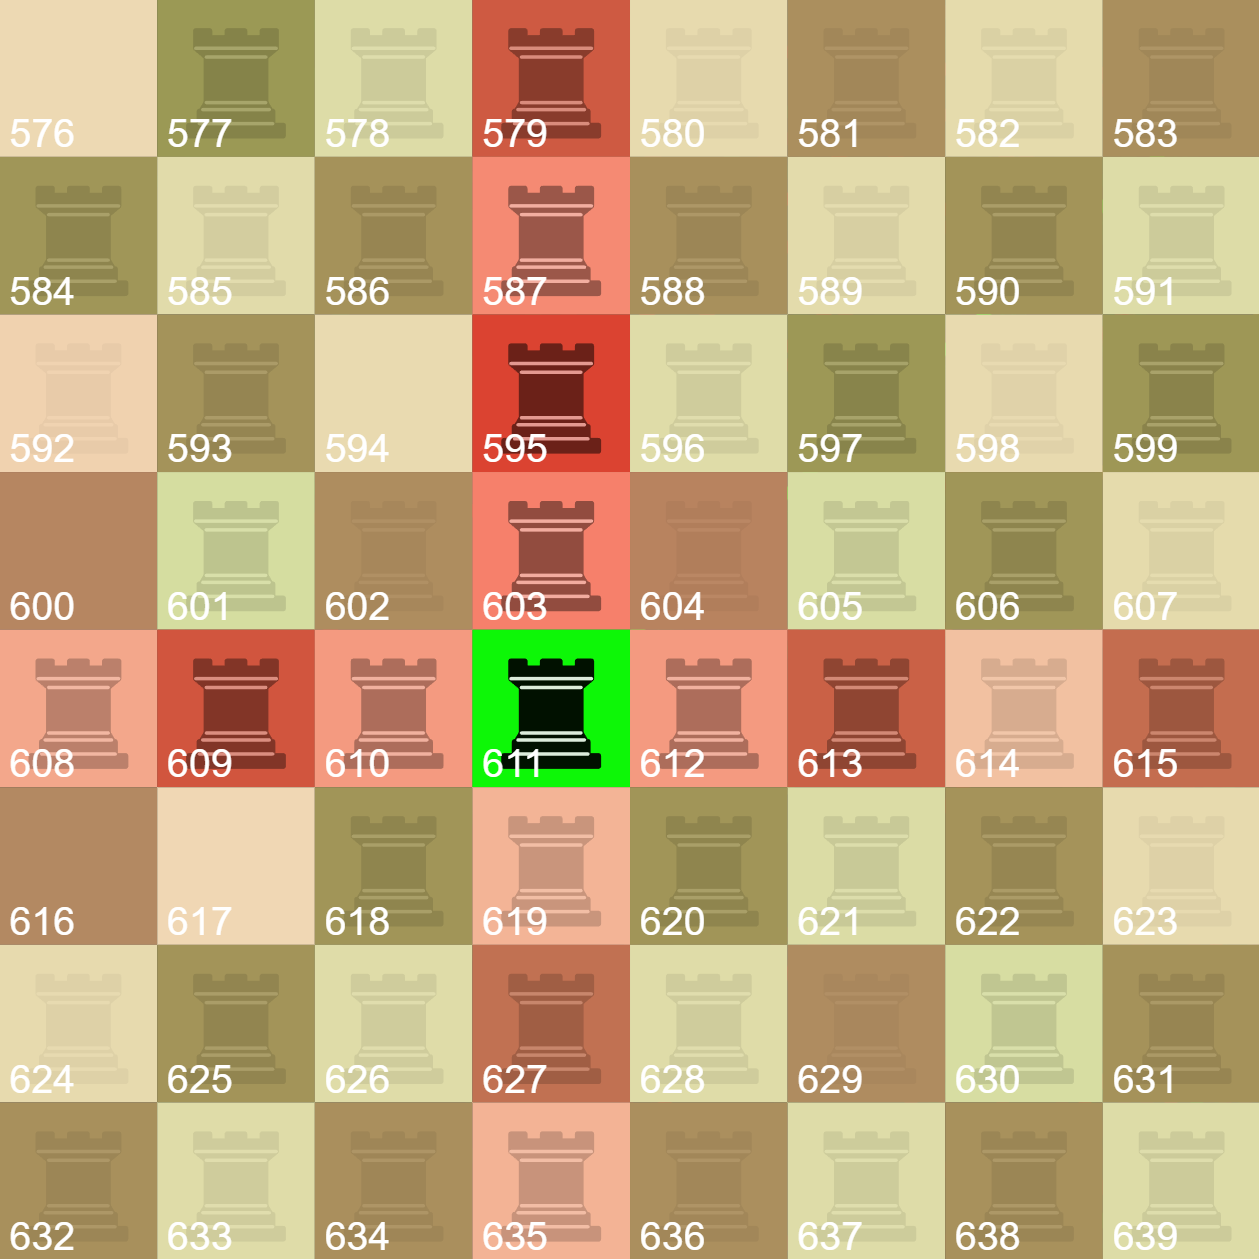
\includegraphics[width=4.4cm]{../assets/results/piece_weights/black_rook_weights.png} }}%
\caption{Weights of \textbf{a neuron} in the L1 layer, which are connected to features in \featureset{All} where the role is $\rook$ Rook. The intensity represents the weight value, and the color represents the sign (although not relevant).}
\label{fig:rook_weights}
\end{figure}

\end{frame}
